\section{Pregunta \texttt{f)}}\label{pregunta-f}

A continuación, nos interesa determinar un equivalente discreto para el
sistema, considerando un tiempo de muestreo $T = 200\ \unit{ms}$.

Para esto, vamos a utilizar las matrices del sistema que obtuvimos en la pregunta
\hyperref[pregunta-b]{\texttt{b)}}:
\begin{align}
    \pmb{A} &= \begin{bmatrix}
        0 & 1 & 0 \\
        -\frac{\nara{a_{0\psi}}}{\nara{a_{2\psi}}}   & -\frac{\nara{a_{1\psi}}}{\nara{a_{2\psi}}} & \frac{\nara{b_{0\psi}}}{\nara{a_{2\psi}}} - \frac{\nara{b_{1\psi}}\nara{a_{0\omega}}}{\nara{a_{2\psi}}\nara{a_{1\omega}}} \\
        0 & 0 & -\frac{\nara{a_{0\omega}}}{\nara{a_{1\omega}}}
    \end{bmatrix} &
    \pmb{B} &= \begin{bmatrix}
        0 \\
        \frac{\nara{b_{1\psi}}\nara{b_{0\omega}}}{\nara{a_{2\psi}}\nara{a_{1\omega}}} \\
        \frac{\nara{b_{0\omega}}}{\nara{a_{1\omega}}}
    \end{bmatrix}
\end{align}
\begin{align}
  \pmb{C} &= \begin{bmatrix}
    1 & 0 & 0
  \end{bmatrix}
\end{align}

De lo visto en el curso de Sistemas Lineales Dinámicos \cite{apunte-sld}, sabemos
que para obtener el equivalente discreto de estas matrices debemos realizar los
siguientes cálculos:
\begin{equation}
\mathbf{A_d}= e^{\mathbf{A}T} ,\quad \mathbf{B_d}= \int_{0}^{T} e^{\mathbf{A}(T-\sigma)}\mathbf{B}  \,d\sigma 
\end{equation}

Nos ayudamos entonces de \textit{MATLAB} para determinar los valores de estas
matrices, y obtenemos:
\begin{align}
    \mathbf{A_d} &= \begin{bmatrix}
        -0.1106 & 0.0970 & 0.7400 \\
        -7.6484 &  -0.2385 & 4.5822 \\
        0 & 0 & 0.7386
    \end{bmatrix} &
    \mathbf{B_d} &= \begin{bmatrix}
        0.0090 \\
        0.0710 \\
        0.0046
    \end{bmatrix}
\end{align}

Además, como la salida del sistema es $\rojo{\psi}$, y no hay perturbaciones,
se tiene que las matrices $\pmb{C_{d}}$ y $\pmb{D_{d}}$ son:
\begin{align}
  \pmb{C_{d}} &= \begin{bmatrix}
      1 & 0 & 0
  \end{bmatrix} &
  \pmb{D_{d}} &= 0
\end{align}

Luego, calculamos los valores propios del sistema. Para esto, se utilizón el
comando \verb|eig| de \textit{MATLAB}, entonces:
\begin{align}
  \lambda_{0} &=  0.7386 \\
  \lambda_{1,2} &=  -0.1745 \pm 0.8588j
\end{align}

A continuación, simularemos el sistema para una entrada
$\verd{v_{i}}(kT) = \frac{\verd{v_{i0}}}{3}\left(r(kT-1) - r(kT-4)\right)$
y un tiempo $0 \leq kT \leq 10\ \unit{s}$, y graficaremos los valores que
toman las variables de estado para esta entrada. Nuevamente nos ayudamos
de \textit{MATLAB}, pero esta vez se utilizó el comando \verb|ss2tf| para
obtener una representación en función de transferencia discreta del sistema,
para luego, con el comando \verb|filter| simular el sistema para la entrada
dada. Además, a diferencia del caso continuo, se utilizó el comando \verb|stem|
en lugar de \verb|plot| para graficar.

El código para realizar los cálculos, simular el sistema y luego graficar está
disponible en el \autoref{lst:problema-f}.

\begin{figure}[h]
  \centering
  % This file was created by matlab2tikz.
%
%The latest updates can be retrieved from
%  http://www.mathworks.com/matlabcentral/fileexchange/22022-matlab2tikz-matlab2tikz
%where you can also make suggestions and rate matlab2tikz.
%
\begin{tikzpicture}

\begin{axis}[%
width=0.856\textwidth,
height=0.159\textheight,
at={(0\textwidth,0.491\textheight)},
scale only axis,
xmin=-0.2,
xmax=10.2,
xlabel style={font=\color{white!15!black}},
xlabel={Tiempo $[\unit{s}]$},
ymin=-1,
ymax=28,
ylabel style={font=\color{white!15!black}},
ylabel={$\verd{v_{i}}(t)\ [\unit{V}]$},
axis background/.style={fill=white},
title style={font=\bfseries},
title={Voltaje del motor}
]
\addplot[ycomb, color=Green, mark=*, mark options={solid, Green}, forget plot] table[row sep=crcr] {%
0	0\\
0.2	0\\
0.4	0\\
0.6	0\\
0.8	0\\
1	0\\
1.2	1.76637280517777\\
1.4	3.53274561035553\\
1.6	5.29911841553329\\
1.8	7.06549122071106\\
2	8.83186402588882\\
2.2	10.5982368310666\\
2.4	12.3646096362444\\
2.6	14.1309824414221\\
2.8	15.8973552465999\\
3	17.6637280517776\\
3.2	19.4301008569554\\
3.4	21.1964736621332\\
3.6	22.9628464673109\\
3.8	24.7292192724887\\
4	26.4955920776665\\
4.2	26.4955920776665\\
4.4	26.4955920776665\\
4.6	26.4955920776665\\
4.8	26.4955920776665\\
5	26.4955920776665\\
5.2	26.4955920776665\\
5.4	26.4955920776665\\
5.6	26.4955920776665\\
5.8	26.4955920776665\\
6	26.4955920776665\\
6.2	26.4955920776665\\
6.4	26.4955920776665\\
6.6	26.4955920776665\\
6.8	26.4955920776665\\
7	26.4955920776665\\
7.2	26.4955920776665\\
7.4	26.4955920776665\\
7.6	26.4955920776665\\
7.8	26.4955920776665\\
8	26.4955920776665\\
8.2	26.4955920776665\\
8.4	26.4955920776665\\
8.6	26.4955920776665\\
8.8	26.4955920776665\\
9	26.4955920776665\\
9.2	26.4955920776665\\
9.4	26.4955920776665\\
9.6	26.4955920776665\\
9.8	26.4955920776665\\
10	26.4955920776665\\
};
\addplot[forget plot, color=white!15!black] table[row sep=crcr] {%
-0.2	0\\
10.2	0\\
};
\end{axis}

\begin{axis}[%
width=0.856\textwidth,
height=0.159\textheight,
at={(0\textwidth,0.246\textheight)},
scale only axis,
xmin=-0.2,
xmax=10.2,
xlabel style={font=\color{white!15!black}},
xlabel={Tiempo $[\unit{s}]$},
ymin=-1,
ymax=32,
ylabel style={font=\color{white!15!black}},
ylabel={$\rojo{\psi}(t)\ [\unit{deg}]$},
axis background/.style={fill=white},
title style={font=\bfseries},
title={Ángulo de la bolita}
]
\addplot[ycomb, color=red, mark=*, mark options={solid, red}, forget plot] table[row sep=crcr] {%
0	0\\
0.2	0\\
0.4	0\\
0.6	0\\
0.8	0\\
1	0\\
1.2	0\\
1.4	0.910544412318189\\
1.6	2.75942525110448\\
1.8	4.12191746763367\\
2	5.33269581165065\\
2.2	7.26484236230358\\
2.4	9.27947095374673\\
2.6	10.8720921159623\\
2.8	12.6674573722958\\
3	14.8039098979972\\
3.2	16.7303813322354\\
3.4	18.5160346413685\\
3.6	20.5474659930397\\
3.8	22.6273676105854\\
4	24.5208611594611\\
4.2	26.4564361194677\\
4.4	27.6204669307599\\
4.6	27.7730891094549\\
4.8	28.3365847049362\\
5	29.1385146843313\\
5.2	29.2499350232072\\
5.4	29.2038073983052\\
5.6	29.583896223164\\
5.8	29.8186873148248\\
6	29.6900373113139\\
6.2	29.7357372991733\\
6.4	29.9523698651762\\
6.6	29.9404543404239\\
6.8	29.8512018463453\\
7	29.9454048849093\\
7.2	30.0208794632032\\
7.4	29.9515814838876\\
7.6	29.9395167662312\\
7.8	30.0129903769541\\
8	30.0084549069398\\
8.2	29.9623549676471\\
8.4	29.98839168436\\
8.6	30.0194827033262\\
8.8	29.9921570960126\\
9	29.9804191621313\\
9.2	30.0074266587043\\
9.4	30.008434761022\\
9.6	29.9883885093047\\
9.8	29.9953862771033\\
10	30.0089123286423\\
};
\addplot[forget plot, color=white!15!black] table[row sep=crcr] {%
-0.2	0\\
10.2	0\\
};
\end{axis}

\begin{axis}[%
width=0.856\textwidth,
height=0.159\textheight,
at={(0\textwidth,0\textheight)},
scale only axis,
xmin=-0.2,
xmax=10.2,
xlabel style={font=\color{white!15!black}},
xlabel={Tiempo $[\unit{s}]$},
ymin=0,
ymax=4.42762378472469,
ylabel style={font=\color{white!15!black}},
ylabel={$\mora{\omega}(t)\ [\unit{RPM}]$},
axis background/.style={fill=white},
title style={font=\bfseries},
title={Velocidad angular del anillo}
]
\addplot[ycomb, color=violet, mark=*, mark options={solid, violet}, forget plot] table[row sep=crcr] {%
0	0\\
0.2	0\\
0.4	0\\
0.6	0\\
0.8	0\\
1	0\\
1.2	0\\
1.4	0.0771677909807976\\
1.6	0.211329915521733\\
1.8	0.387586727712501\\
2	0.594933696023216\\
2.2	0.825243129707313\\
2.4	1.07251210563332\\
2.6	1.33230700455488\\
2.8	1.60135325853383\\
3	1.87723234793961\\
3.2	2.15815801048851\\
3.4	2.44281095445107\\
3.6	2.73021678167569\\
3.8	3.01965582437657\\
4	3.31059655268463\\
4.2	3.60264639101527\\
4.4	3.81834760120209\\
4.6	3.97765949242587\\
4.8	4.09532354569344\\
5	4.18222747561982\\
5.2	4.24641269469839\\
5.4	4.29381840295178\\
5.6	4.32883115522197\\
5.8	4.35469075877395\\
6	4.37379005981447\\
6.2	4.38789635883423\\
6.4	4.3983149428239\\
6.6	4.4060098663611\\
6.8	4.41169315770876\\
7	4.41589070436223\\
7.2	4.41899091458028\\
7.4	4.42128065765868\\
7.6	4.42297180857953\\
7.8	4.42422085327109\\
8	4.42514336859616\\
8.2	4.42582471693442\\
8.4	4.42632794495181\\
8.6	4.42669961744774\\
8.8	4.42697412609881\\
9	4.42717687179654\\
9.2	4.42732661504793\\
9.4	4.42743721192663\\
9.6	4.42751889620597\\
9.8	4.42757922631267\\
10	4.42762378472469\\
};
\addplot[forget plot, color=white!15!black] table[row sep=crcr] {%
-0.2	0\\
10.2	0\\
};
\end{axis}
\end{tikzpicture}%

  \caption{Variables de estado del sistema discreto}\label{fig:estado-discreto}
\end{figure}

\subsection{Comentarios}

Aqui van a ir los comentarios \textbf{NO OLVIDAR!!}.
